%%%
%%% Informations
%%%
\documentclass{beamer}
\title{Un détecteur d'obstacles pour malvoyants}
\subtitle{Santé et prévention}
\author{Arthur Jacquin}
\institute{Candidat 27397}
\date{}



%%%
%%% Configuration
%%%

% Couleurs
\usepackage{xcolor}
\definecolor{beaverred}{RGB}{204,0,0}
\definecolor{beaverblue}{RGB}{0,68,204}
\definecolor{beavergreen}{RGB}{0,153,0}

% Figures
\usepackage{caption}
\DeclareCaptionFont{captioncolor}{\color{beaverred}}
\captionsetup{labelfont={captioncolor}}
\DeclareCaptionLabelSeparator{sep}{ : }
\captionsetup{labelsep=sep}
\usepackage{subfig}
\usepackage{tikz}
\usepackage{circuitikz}
\usepackage{pgfplots}
\pgfkeys{/pgf/number format/.cd,1000 sep={\,}}
\pgfplotsset{width=8cm,compat=1.9}

% Code
\usepackage{listings}
\lstdefinestyle{simple}{
    extendedchars=true,
    basicstyle=\ttfamily,
    backgroundcolor=,
    commentstyle=\color{beavergreen},
    keywordstyle=\color{beaverblue},
    numberstyle=\ttfamily\color[rgb]{0.5,0.5,0.5},
    breakatwhitespace=false,
    breaklines=true,
    captionpos=b,
    keepspaces=true,
    numbers=left,
    numbersep=7pt,
    showspaces=false,
    showstringspaces=false,
    showtabs=false,
    tabsize=4,
    columns=fixed
}
\lstset{style=simple}

% Thème
\usetheme{default}
\usecolortheme{beaver}
\setbeamertemplate{navigation symbols}{}
\setbeamertemplate{footline}[frame number]
\setbeamertemplate{itemize items}{\color{beaverred}$\bullet$}
\setbeamertemplate{caption}[numbered]



%%%
%%% Début du document
%%%
\begin{document}



%%%
%%% Page de titre
%%%
\frame{\titlepage}



%%%
%%% Sommaire
%%%
\begin{frame}
\frametitle{Sommaire}
\begin{itemize}
\item Introduction
\item Capteurs de distance
\item Interface utilisateur
\item Produit fini
\item Annexes
\end{itemize}
\end{frame}



%%%
%%% Contexte
%%%
\begin{frame}
\frametitle{Introduction - Contexte}
\begin{itemize}
% Nombre d'aveugles, impact sur la mobilité
% Relier au thème Santé et prévention
\item Solutions existantes partiellement satisfaisantes
    \begin{itemize}
    \item Chiens-guides
    \item Cannes
    \item Cannes électroniques
    \end{itemize}
\end{itemize}
\begin{center}
\begin{figure}
\includegraphics[height=4cm]{images/ultracane.jpg}
\caption{L'UltraCane (CECIAA, 1055 €)}
\end{figure}
\end{center}
\end{frame}
% Objectif : concevoir un détecteur d'obstacles personnel



%%%
%%% Problématique
%%%
\begin{frame}
\frametitle{Introduction - Problématique}
\begin{center}
Peut-on proposer une meilleure alternative ?
\end{center}
\end{frame}



%%%
%%% Cahier des charges fonctionnel
%%%
\begin{frame}
\frametitle{Introduction - Cahier des charges fonctionnel}
\begin{center}
\begin{tabular}{llc}
\hline
{\bf Fonction} & {\bf Critère} & {\bf Valeur} \\
\hline
Détecter la distance de & Portée & \textgreater 3 m \\
l'obstacle le plus proche & Faisceau de détection & \\
 & Réactivité & \textgreater 5 Hz \\
\hline
Traiter l'information & Cohérence & \\
\hline
Communiquer l'information & Clarté & \\
à l'utilisateur & Progressivité & \\
\hline
Être reproductible & Accessibilité économique & \textless 50 € \\
 & Accessibilité technique & \\
\hline
Être ergonomique & Compacité & \\
 & Maniabilité & \\
 & Robustesse & \\
\hline
\end{tabular}
\end{center}
\end{frame}
% Parler du dispositif envisagé
% microcontrôleur grand public
% Mode balayage -> pas de pbms d'obstacle hauts



%%%
%%% Capteurs de distance
%%%
\begin{frame}
\frametitle{Capteurs de distance - Modèles}
% Echolocalisation, biomimétisme, observation des chauves souris, dauphins, ...
\begin{tabular}{r|ccc}
{\bf Capteur} & VL53L1X & \multicolumn{2}{c}{MB1013} \\
 & \includegraphics[height=2cm]{images/VL53L1X.jpg} & \multicolumn{2}{c}{\includegraphics[height=2cm]{images/maxsonar_ez1_mb1013.jpg}} \\
{\bf Type d'onde} & Lumineuse & \multicolumn{2}{c}{Sonore} \\
{\bf Domaine} & Infrarouge (940 nm) & \multicolumn{2}{c}{Ultrasonore (42 kHz)} \\
% Laser de classe 1 -> innofensif
{\bf Prix} & 19,40 € & \multicolumn{2}{c}{39,90 €} \\
{\bf Interface} & I²C & Analogique & MLA \\
% Parler du I2C, on y reviendra tout à l'heure pour le MLA
 &
    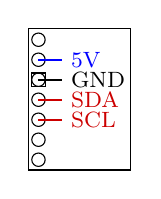
\begin{tikzpicture}
    \footnotesize
    \draw (0, 0) rectangle (1.3, 1.8);
    \foreach \y in {0.13,0.384,...,1.8} \draw (0.13, \y) circle (0.085);
    \draw (0.045, 1.061) rectangle (0.215, 1.231);
    \draw[color=blue, thick] (0.13, 1.4) -- +(0.3,0) node[anchor=west] {5V};
    \draw[color=black, thick] (0.13, 1.146) -- +(0.3,0) node[anchor=west] {GND};
    \draw[color=beaverred, thick] (0.13, 0.892) -- +(0.3,0) node[anchor=west] {SDA};
    \draw[color=beaverred, thick] (0.13, 0.638) -- +(0.3,0) node[anchor=west] {SCL};
    \end{tikzpicture}
    &
    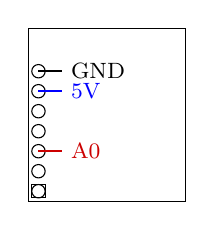
\begin{tikzpicture}
    \footnotesize
    \draw (0, 0) rectangle (2, 2.2);
    \foreach \y in {0.13,0.384,...,1.8} \draw (0.13, \y) circle (0.085);
    \draw (0.045, 0.045) rectangle (0.215, 0.215);
    \draw[color=black, thick] (0.13, 1.654) -- +(0.3,0) node[anchor=west] {GND};
    \draw[color=blue, thick] (0.13, 1.4) -- +(0.3,0) node[anchor=west] {5V};
    \draw[color=beaverred, thick] (0.13, 0.638) -- +(0.3,0) node[anchor=west] {A0};
    \end{tikzpicture}
    & 
    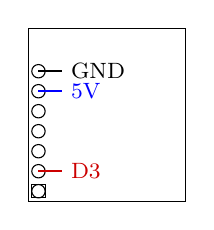
\begin{tikzpicture}
    \footnotesize
    \draw (0, 0) rectangle (2, 2.2);
    \foreach \y in {0.13,0.384,...,1.8} \draw (0.13, \y) circle (0.085);
    \draw (0.045, 0.045) rectangle (0.215, 0.215);
    \draw[color=black, thick] (0.13, 1.654) -- +(0.3,0) node[anchor=west] {GND};
    \draw[color=blue, thick] (0.13, 1.4) -- +(0.3,0) node[anchor=west] {5V};
    \draw[color=beaverred, thick] (0.13, 0.384) -- +(0.3,0) node[anchor=west] {D3};
    \end{tikzpicture} \\
\end{tabular}
\end{frame}



%%%
%%% Faisceau de détection
%%%
\begin{frame}
\frametitle{Capteurs de distance - Faisceau de détection}
% Diamètre du poteau: 6 cm
% Côté du coussin: 35 cm
\begin{figure}
\centering
\subfloat[\centering Dispositif]{{\includegraphics[height=6cm]{images/faisceau.jpg}}}
\quad
\subfloat[\centering Zone détectée par le capteur placé à l'origine (vue de haut, en m)]{{
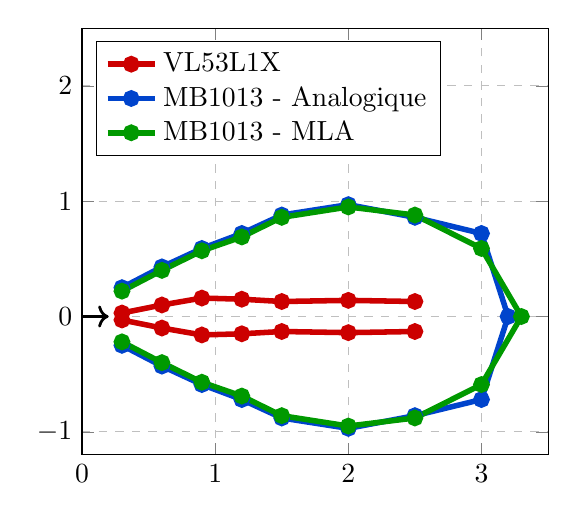
\begin{tikzpicture}
\begin{axis}[
    legend cell align = {left},
    legend pos=north west,
    width=7.5cm,
    height=7cm,
    xmin=0, xmax=3.5,
    ymin=-1.2, ymax=2.5,
    xtick distance=1,
    ytick distance=1,
    grid=both,
    grid style=dashed,
]
\addplot[line width=2pt, color=beaverred, mark=*] coordinates {
    (2.5,-0.13)(2,-0.14)(1.5,-0.13)(1.2,-0.15)(0.9,-0.16)(0.6,-0.10)
    (0.3,-0.03)(0.3,0.03)(0.6,0.10)(0.9,0.16)(1.2,0.15)(1.5,0.13)(2,0.14)(2.5,0.13)};
\addplot[line width=2pt, color=beaverblue, mark=*] coordinates {
    (0.3,0.25)(0.6,0.43)(0.9,0.59)(1.2,0.72)(1.5,0.88)(2,0.97)
    (2.5,0.86)(3,0.72)(3.2,0)(3,-0.72)(2.5,-0.86)(2,-0.97)(1.5,-0.88)
    (1.2,-0.72)(0.9,-0.59)(0.6,-0.43)(0.3,-0.25)};
\addplot[line width=2pt, color=beavergreen, mark=*] coordinates {
    (0.3,0.22)(0.6,0.40)(0.9,0.57)(1.2,0.69)(1.5,0.86)(2,0.95)(2.5,0.88)
    (3,0.59)(3.3,0)(3,-0.59)(2.5,-0.88)(2,-0.95)(1.5,-0.86)
    (1.2,-0.69)(0.9,-0.57)(0.6,-0.40)(0.3,-0.22)};
\legend{
    VL53L1X,
    MB1013 - Analogique,
    MB1013 - MLA}
\draw[line width=1pt,->] (axis cs:0,0) -- (axis cs:0.2,0);
\end{axis}
\end{tikzpicture}
}}
\caption{Faisceau de détection}
\end{figure}
% Conclure sur la cohérence: laser unidimensionnelle, onde sonore tridimensionnelle
\end{frame}



%%%
%%% Précision
%%%
\begin{frame}
\frametitle{Capteurs de distance - Précision}
\begin{center}
\begin{figure}
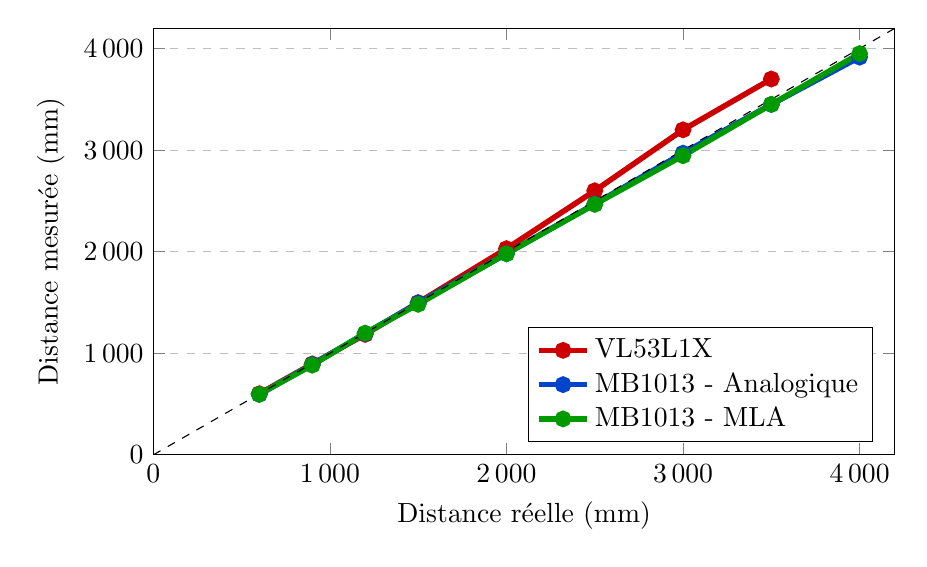
\begin{tikzpicture}
\begin{axis}[
    width=11cm,
    height=7cm,
    xlabel={Distance réelle (mm)},
    ylabel={Distance mesurée (mm)},
    xmin=0, xmax=4200,
    ymin=0, ymax=4200,
    xtick={0,1000,2000,3000,4000},
    ytick={0,1000,2000,3000,4000},
    legend cell align = {left},
    legend pos=south east,
    ymajorgrids=true,
    grid style=dashed,
]
\addplot[color=beaverred, line width=2pt, mark=*]
    coordinates {(600,602)(900,895)(1200,1186)(1500,1499)
        (2000,2030)(2500,2600)(3000,3200)(3500,3700)};
\addplot[color=beaverblue, line width=2pt, mark=*]
    coordinates {(600,595)(900,890)(1200,1195)(1500,1495)
        (2000,1980)(2500,2470)(3000,2970)(3500,3450)(4000,3915)};
\addplot[color=beavergreen, line width=2pt, mark=*]
    coordinates {(600,597)(900,883)(1200,1198)(1500,1482)
        (2000,1980)(2500,2466)(3000,2945)(3500,3450)(4000,3950)};
\addplot[dashed] coordinates {(0,0)(4200,4200)};
\legend{
    VL53L1X,
    MB1013 - Analogique,
    MB1013 - MLA}
\end{axis}
\end{tikzpicture}
\caption{Mesures de distance}
\end{figure}
\end{center}
\end{frame}



%%%
%%% Réactivité
%%%
\begin{frame}
\frametitle{Capteurs de distance - Réactivité}
\begin{center}
\begin{figure}
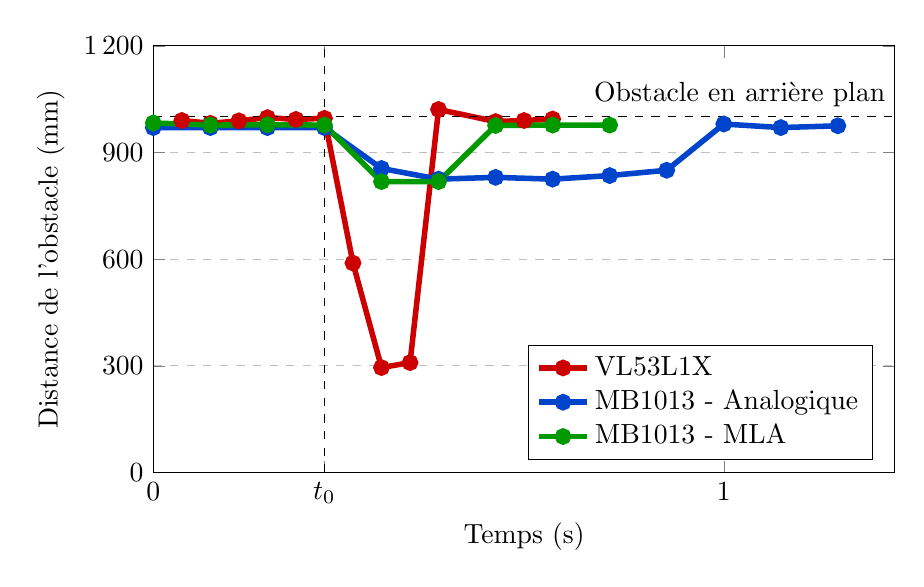
\begin{tikzpicture}
\begin{axis}[
    width=11cm,
    height=7cm,
    xlabel={Temps (s)},
    ylabel={Distance de l'obstacle (mm)},
    xmin=0, xmax=1.3,
    ymin=0, ymax=1200,
    xtick={0, 0.3, 1},
    xticklabels = {0, $t_0$, 1},
    ytick={0, 300, 600, 900, 1200},
    legend cell align = {left},
    legend pos=south east,
    ymajorgrids=true,
    grid style=dashed,
]
\addplot[color=beaverred, line width=2pt, mark=*]
    coordinates {(0.05,990)(0.1,982)(0.15,989)(0.2,998)
        (0.25,993)(0.3,996)(0.35,589)(0.4,295)(0.45,309)
        (0.5,1021)(0.6,987)(0.65,990)(0.7,994)};
\addplot[color=beaverblue, line width=2pt, mark=*]
    coordinates {(0,970)(0.1,970)(0.2,970)(0.3,970)
        (0.4,855)(0.5,825)(0.6,830)(0.7,825)(0.8,835)
        (0.9,850)(1,980)(1.1,970)(1.2,975)};
\addplot[color=beavergreen, line width=2pt, mark=*]
    coordinates {(0,983)(0.1,977)(0.2,978)(0.3,977)
        (0.4,818)(0.5,818)(0.6,976)(0.7,977)(0.8,977)};
\addplot[dashed] coordinates {(0,1000)(1.3,1000)};
\node at (axis cs:1.3,1000) [anchor=south east] {Obstacle en arrière plan};
\addplot[dashed] coordinates {(0.3,0)(0.3,1200)};
\legend{
    VL53L1X,
    MB1013 - Analogique,
    MB1013 - MLA}
\end{axis}
\end{tikzpicture}
\caption{Détection d'une feuille A4 lachée à 30 cm du capteur à $t_0$}
\end{figure}
\end{center}
\end{frame}



%%%
%%% Conclusion
%%%
\begin{frame}
\frametitle{Capteurs de distance - Conclusion}
\begin{itemize}
\item Récapitulatif des tests
\end{itemize}
\begin{center}
% Préciser: mode de communication du MB1013 peu significatif
\begin{tabular}{r|cc}
{\bf Capteur} & VL53L1X & MB1013 \\
{\bf Portée} & ++ & +++ \\ 
{\bf Faisceau} & Directif & Large \\
{\bf Précision} & Suffisante & Suffisante \\
{\bf Réactivité} & +++ & + \\
{\bf Prix} & 19,40 € & 39,90 € \\
\end{tabular}
\end{center}
% S'appuyer sur un fonctionnement par balayage
\begin{itemize}
\item Capteur retenu : VL53L1X
\item Léger bruit : moyenne glissante sur 3 points (0,15 s)
% Un traitement du signal plus poussé a été envisagé (eg filtre de Kalman) mais abandonné à cause des limitations techniques et du besoin de réactivité
\end{itemize}
\end{frame}



%%%
%%% Interface utilisateur
%%%
\begin{frame}
\frametitle{Interface utilisateur - Modèles}
\begin{itemize}
\item Signal sonore : désagréable
\item Vibrations : comparaison de différents vibreurs
\end{itemize}
\bigskip
\begin{tabular}{cccc}
Vibreur Gotronic & VPM2 & Gravity & SMD \\
  \includegraphics[width=2.3cm]{images/gotronic_vib.jpg}
& \includegraphics[width=2.3cm]{images/vpm2.jpg}
& \includegraphics[width=2.3cm]{images/gravity.jpg}
& \includegraphics[width=2.3cm]{images/smd.jpg} \\
1,30 € & 4,20 € & 2,60 € & 1,30 € \\
\end{tabular}
\end{frame}



%%%
%%% Modulation de largeur d'amplitude
%%%
\begin{frame}
\frametitle{Interface utilisateur - Modulation de largeur d'amplitude}
\begin{itemize}
\item {\it Pulse Width Modulation} ({\it PWM})
\item Caractérisé par le rapport cyclique ({\it duty cycle}) noté $D = \frac{T_{on}}{T}$
\end{itemize}
\begin{center}
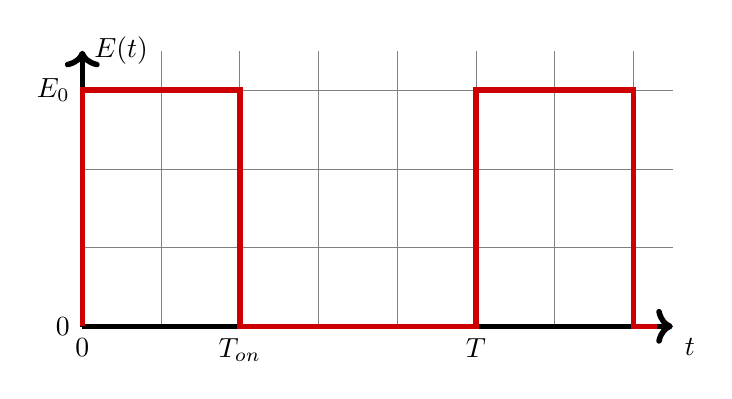
\begin{tikzpicture}
\draw[step=1cm,gray,very thin] (0,0) grid (7.5,3.5);
\draw[->, line width=2pt] (0,0) -- (0,3.5) node[anchor=west] {$E(t)$};
\draw (1pt,0) -- (-1pt,0) node[anchor=east] {$0$};
\draw (1pt,3) -- (-1pt,3) node[anchor=east] {$E_0$};
\draw[->, line width=2pt] (0,0) -- (7.5,0) node[anchor=north west] {$t$};
\draw (0,1pt) -- (0,-1pt) node[anchor=north] {$0$};
\draw (2,1pt) -- (2,-1pt) node[anchor=north] {$T_{on}$};
\draw (5,1pt) -- (5,-1pt) node[anchor=north] {$T$};
\draw[color=beaverred, line width=2pt] (0,0) -- (0,3) -- (2,3) -- (2,0)
    -- (5,0) -- (5,3) -- (7,3) -- (7,0) -- (7.3,0);
\end{tikzpicture}
$$<E(t)> \;
    = \frac{1}{T} \int_0^T{E(t) \: dt}
    = \frac{1}{T} \left(\int_0^{T_{on}}{E_0 \: dt} + \int_{T_{on}}^T{0 \: dt} \right)
    = D \cdot E_0$$
\end{center}
\end{frame}
% La première question qui se pose est la façon dont on fait varier l'intensité
% de la vibration. En effet, on aimerait une amplitude de vibration décroissante
% avec la distance de l'obstacle, mais le microcontrôleur ne permet que de fixer
% une tension maximale $E_0$ ou nulle.

% Pour simuler un signal analogique, à valeurs dans une plage continue de données,
% à partir d'un ensemble discret de valeurs, on utilise le principe de modulation
% de largeur d'amplitude.
% Les vibreurs se comportant comme des filtres passe-bas, on effectue une
% succession assez de valeurs à ces états discrets, de façon à obtenir une
% composante continue, c'est à dire la moyenne du signal, à la tension souhaitée.
% Le microcontrôleur permet de générer de tels signaux à une fréquence de 490Hz.

% Description, ici rapport cyclique de 40% ... Après calcul, simple relation de
% Chasles, la moyenne temporelle de la tension est proportionnelle au rapport cyclique.

% Retour sur mode MLA du Maxbotic



%%%
%%% Courbes intensité-ressenti
%%%
\begin{frame}
\frametitle{Interface utilisateur - Courbes intensité-ressenti}
% Tension minimale de mise en route (réel et non idéaux)
% Ressenti a priori non proportionnel à la tension
\begin{center}
\begin{figure}
\subfloat[\centering Vibreur Gotronic]{
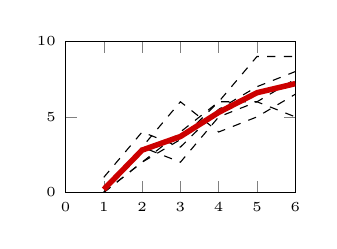
\begin{tikzpicture}
\begin{axis}[width=4.5cm, height=3.5cm, xmin=0, xmax=6, ymin=0, ymax=10,
    xtick distance=1, ytick distance=5, ticklabel style = {font=\tiny}]
\addplot[dashed, mark=none] coordinates {(1,0)(2,3)(3,2)(4,5)(5,6)(6,7.5)};
\addplot[dashed, mark=none] coordinates {(1,1)(2,4)(3,3)(4,5.5)(5,7)(6,8)};
\addplot[dashed, mark=none] coordinates {(1,0)(2,3)(3,6)(4,4)(5,5)(6,6.5)};
\addplot[dashed, mark=none] coordinates {(1,0)(2,2)(3,4)(4,6)(5,9)(6,9)};
\addplot[dashed, mark=none] coordinates {(1,0)(2,2)(3,3.5)(4,6)(5,6)(6,5)};
\addplot[line width=2pt, color=beaverred, mark=none] coordinates {(1,0.2)(2,2.8)(3,3.7)(4,5.3)(5,6.6)(6,7.2)};
\end{axis}
\end{tikzpicture}}
\quad
\subfloat[\centering VPM2]{
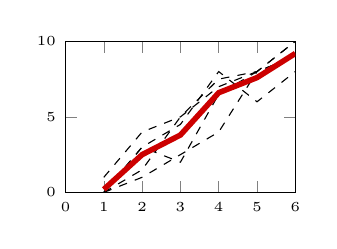
\begin{tikzpicture}
\begin{axis}[width=4.5cm, height=3.5cm, xmin=0, xmax=6, ymin=0, ymax=10,
    xtick distance=1, ytick distance=5, ticklabel style = {font=\tiny}]
\addplot[dashed, mark=none] coordinates {(1,0)(2,3)(3,2)(4,6.5)(5,8)(6,9)};
\addplot[dashed, mark=none] coordinates {(1,1)(2,4)(3,5)(4,7)(5,8)(6,9)};
\addplot[dashed, mark=none] coordinates {(1,0)(2,3)(3,4.5)(4,8)(5,6)(6,8)};
\addplot[dashed, mark=none] coordinates {(1,0)(2,1)(3,2.5)(4,4)(5,8)(6,10)};
\addplot[dashed, mark=none] coordinates {(1,0)(2,1.5)(3,5)(4,7.5)(5,8)(6,10)};
\addplot[line width=2pt, color=beaverred, mark=none] coordinates {(1,0.2)(2,2.5)(3,3.8)(4,6.6)(5,7.6)(6,9.2)};
\end{axis}
\end{tikzpicture}}
\quad
\subfloat[\centering Gravity]{
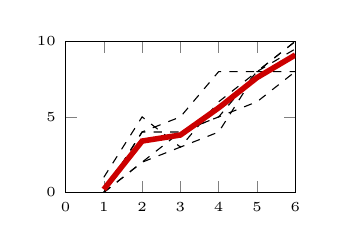
\begin{tikzpicture}
\begin{axis}[width=4.5cm, height=3.5cm, xmin=0, xmax=6, ymin=0, ymax=10,
    xtick distance=1, ytick distance=5, ticklabel style = {font=\tiny}]
\addplot[dashed, mark=none] coordinates {(1,0)(2,2)(3,3)(4,6)(5,8)(6,9.5)};
\addplot[dashed, mark=none] coordinates {(1,0)(2,4)(3,5)(4,8)(5,8)(6,10)};
\addplot[dashed, mark=none] coordinates {(1,1)(2,5)(3,3)(4,4)(5,8)(6,8)};
\addplot[dashed, mark=none] coordinates {(1,0)(2,2)(3,4)(4,5)(5,6)(6,8)};
\addplot[dashed, mark=none] coordinates {(1,0)(2,4)(3,4)(4,5)(5,8)(6,10)};
\addplot[line width=2pt, color=beaverred, mark=none] coordinates {(1,0.2)(2,3.4)(3,3.8)(4,5.6)(5,7.6)(6,9.1)};
\end{axis}
\end{tikzpicture}}
\quad
\subfloat[\centering SMD]{
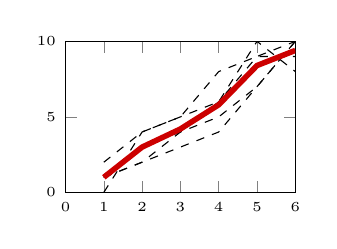
\begin{tikzpicture}
\begin{axis}[width=4.5cm, height=3.5cm, xmin=0, xmax=6, ymin=0, ymax=10,
    xtick distance=1, ytick distance=5, ticklabel style = {font=\tiny}]
\addplot[dashed, mark=none] coordinates {(1,0)(2,4)(3,5)(4,8)(5,9)(6,9)};
\addplot[dashed, mark=none] coordinates {(1,1)(2,3)(3,4)(4,5)(5,7)(6,10)};
\addplot[dashed, mark=none] coordinates {(1,1)(2,2)(3,3)(4,4)(5,7)(6,10)};
\addplot[dashed, mark=none] coordinates {(1,1)(2,2)(3,4)(4,6)(5,9)(6,10)};
\addplot[dashed, mark=none] coordinates {(1,2)(2,4)(3,5)(4,6)(5,10)(6,8)};
\addplot[line width=2pt, color=beaverred, mark=none] coordinates {(1,1)(2,3)(3,4.2)(4,5.8)(5,8.4)(6,9.4)};
\end{axis}
\end{tikzpicture}}
\caption{Intensité de vibration ressentie en fonction de l’intensité des vibrations (5 utilisateurs en pointillés, moyenne en rouge)}
\end{figure}
\end{center}
\end{frame}
% Choix du vibreur B
    % Facile à utiliser, assez puissant, relativement cohérent


%%%
%%% Modélisation de la courbe intensité-ressenti
%%%
\begin{frame}
\frametitle{Interface utilisateur - Fonction \lstinline+dist_to_intensity+}
\begin{center}
\[ f(x) = \begin{cases}
    a x^3 + b x^2 + b x + d & x \leq 2000 \\
    0 & x > 2000
\end{cases}\]
\[
    (a, b, c, d) =  (-1.8 \cdot 10^{-8}, \; 1.08 \cdot 10^{-4}, \; -0.234, \; 255)
\]
% Modélisation
    % Prends une distance en mm, Retour entre 0 et 255
    % Simple pour calcul rapide
    % Exploiter au mieux l'étendue de la plage d'intensité ressentie de vibration
    % Fonction polynomiale de degré 3 convient
\begin{figure}
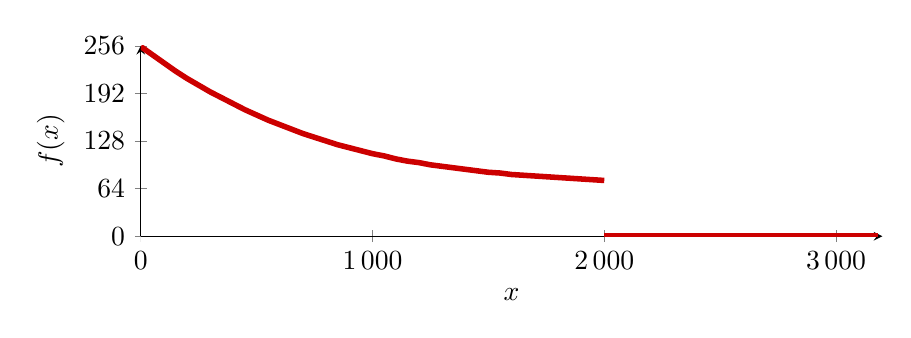
\begin{tikzpicture}
\begin{axis}[
    xlabel = $x$,
    ylabel = {$f(x)$},
    axis lines = left,
    width=11cm,
    height=4cm,
    xmin=0, xmax=3200,
    ymin=0, ymax=256,
    xtick distance=1000,
    ytick distance=64,
]
\addplot[color=beaverred, line width=2pt]
    coordinates{(0,255)(50,244)(100,233)(150,222)(200,212)
        (250,203)(300,194)(350,186)(400,178)(450,170)(500,163)
        (550,156)(600,150)(650,144)(700,138)(750,133)(800,128)
        (850,123)(900,119)(950,115)(1000,111)(1050,108)(1100,104)
        (1150,101)(1200,99)(1250,96)(1300,94)(1350,92)(1400,90)
        (1450,88)(1500,86)(1550,85)(1600,83)(1650,82)(1700,81)
        (1750,80)(1800,79)(1850,78)(1900,77)(1950,76)(2000,75)};
\addplot[color=beaverred, line width=2pt]
    coordinates{(2000,0)(3180,0)};
\end{axis}
\end{tikzpicture}
\caption{Fonction \lstinline+dist_to_intensity+}
\end{figure}
% On retrouve la tension minimale de mise en route
\end{center}
\end{frame}



%%%
%%% Conception générale
%%%
\begin{frame}
\frametitle{Produit fini - Conception générale}
\begin{itemize}
\item Choix du microcontrôleur
% Arduino Nano Every ->
%   très populaire
%   pas cher
%   la board la plus compacte de chez Arduino
%   convient: interface I²C, tension de 5V sur les I/O pins
% D'autres, plus petites envisagées, mais pas assez de tension sur I/O pins
\item Alimentation : externe
% dispositif externe
% plus maniable
% flexibilité pour l'utilisateur, qui peut utiliser plusieurs batteries externes,
%     et alimentation avec un câble micro-USB
% supprime le besoin d'un interrupteur de mise sous tension: on branche et on débranche
\item Nombre de couples capteur-vibreur : un seul
% Correspond au mode balayage, plus clair pour l'utilisateur
% Simplifie la fabrication et permet de garder un prix attractif
% -> rejoint l'objectif de reproducibilité
\item Boîtier : aucun
% Initiallement, dessin puis impression 3D d'un boitier envisagé. Mais:
% 1. Nuit à la reproducibilité
% 2. Le rendu étant très compact, les éléments sont fixes les uns aux autres, pas de fil
%    qui dépasse -> pas besoin de boîtier
\item Disposition générale des composants
% que je commenterai avec les images
\end{itemize}
\end{frame}



%%%
%%% Composants
%%%
\begin{frame}
\frametitle{Produit fini - Composants}
\begin{itemize}
\item Composants retenus
\end{itemize}
\begin{center}
\begin{tabular}{ccr}
\hline
{\bf Composant} & {\bf Nom} & {\bf Prix (€)} \\
\hline
Microcontrôleur & Arduino Nano Every & 8,80 \\
Capteur de distance & VL53L1X & 19,40 \\
Vibreur & VPM2 & 4,20 \\
\hline
\multicolumn{2}{r}{\bf TOTAL} & 32,40 \\
\hline
\end{tabular}
\end{center}
\begin{itemize}
\item Matériel nécessaire
    \begin{itemize}
    \item Station de soudure
    % Seulement 10 points de soudures, 4 bouts de fils: accessible
    \item Scotch double face
    \item Fils de prototypage
    \end{itemize}
\end{itemize}
\end{frame}



%%%
%%% Schéma
%%%
\begin{frame}
\frametitle{Produit fini - Schéma de soudure}
\begin{center}
\begin{figure}
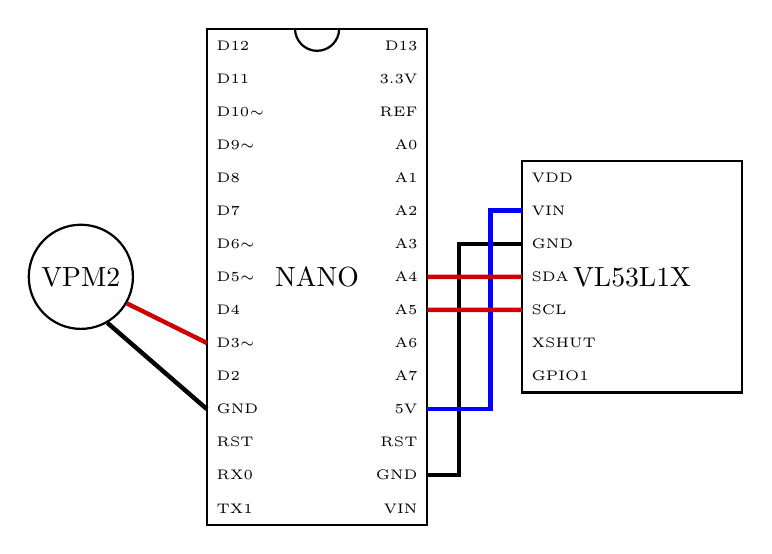
\begin{tikzpicture}
% Configuration
\ctikzset{multipoles/dipchip/pin spacing=0.3}
\ctikzset{multipoles/external pins width=0}
\ctikzset{multipoles/dipchip/width=2}

% NANO
\node[dipchip, num pins=30, hide numbers] (N) at (0, 0) {NANO};
\node[font=\tiny, right] at (N.bpin 1) {D12};
\node[font=\tiny, right] at (N.bpin 2) {D11};
\node[font=\tiny, right] at (N.bpin 3) {D10$\sim$};
\node[font=\tiny, right] at (N.bpin 4) {D9$\sim$};
\node[font=\tiny, right] at (N.bpin 5) {D8};
\node[font=\tiny, right] at (N.bpin 6) {D7};
\node[font=\tiny, right] at (N.bpin 7) {D6$\sim$};
\node[font=\tiny, right] at (N.bpin 8) {D5$\sim$};
\node[font=\tiny, right] at (N.bpin 9) {D4};
\node[font=\tiny, right] at (N.bpin 10) {D3$\sim$};
\node[font=\tiny, right] at (N.bpin 11) {D2};
\node[font=\tiny, right] at (N.bpin 12) {GND};
\node[font=\tiny, right] at (N.bpin 13) {RST};
\node[font=\tiny, right] at (N.bpin 14) {RX0};
\node[font=\tiny, right] at (N.bpin 15) {TX1};
\node[font=\tiny, left] at (N.bpin 16) {VIN};
\node[font=\tiny, left] at (N.bpin 17) {GND};
\node[font=\tiny, left] at (N.bpin 18) {RST};
\node[font=\tiny, left] at (N.bpin 19) {5V};
\node[font=\tiny, left] at (N.bpin 20) {A7};
\node[font=\tiny, left] at (N.bpin 21) {A6};
\node[font=\tiny, left] at (N.bpin 22) {A5};
\node[font=\tiny, left] at (N.bpin 23) {A4};
\node[font=\tiny, left] at (N.bpin 24) {A3};
\node[font=\tiny, left] at (N.bpin 25) {A2};
\node[font=\tiny, left] at (N.bpin 26) {A1};
\node[font=\tiny, left] at (N.bpin 27) {A0};
\node[font=\tiny, left] at (N.bpin 28) {REF};
\node[font=\tiny, left] at (N.bpin 29) {3.3V};
\node[font=\tiny, left] at (N.bpin 30) {D13};

% VL53L1X
\node[dipchip, num pins=14, hide numbers, no topmark] (C) at (4, 0) {VL53L1X};
\node[font=\tiny, right] at (C.bpin 1) {VDD};
\node[font=\tiny, right] at (C.bpin 2) {VIN};
\node[font=\tiny, right] at (C.bpin 3) {GND};
\node[font=\tiny, right] at (C.bpin 4) {SDA};
\node[font=\tiny, right] at (C.bpin 5) {SCL};
\node[font=\tiny, right] at (C.bpin 6) {XSHUT};
\node[font=\tiny, right] at (C.bpin 7) {GPIO1};

% VPM2
\node[circle, thick, draw] (V) at (-3,0) {VPM2};

% Connections
\draw[color=black, ultra thick] (N.pin 17) -- +(0.4,0) |- (C.pin 3);
\draw[color=blue, ultra thick] (C.pin 2) -- +(-0.4,0) |- (N.pin 19);
\draw[color=beaverred, ultra thick] (N.pin 23) -- (C.pin 4);
\draw[color=beaverred, ultra thick] (N.pin 22) -- (C.pin 5);
\draw[color=black, ultra thick] (V.-60) -- (N.pin 12);
\draw[color=beaverred, ultra thick] (V.-30) -- (N.pin 10);
\end{tikzpicture}
\caption{Schéma de soudure}
\end{figure}
\end{center}
\end{frame}



%%%
%%% Produit fini
%%%
\begin{frame}
\frametitle{Produit fini - Conclusion}
\begin{figure}
\centering
\subfloat[\centering Vue de face]{{\includegraphics[height=5cm]{images/produit_fini.jpg}}}
\qquad
\subfloat[\centering Dans la main]{{\includegraphics[height=5cm]{images/produit_fini_main.jpg}}}
\caption{Produit fini}
\end{figure}
\begin{itemize}
\item Documentation disponible en ligne
\end{itemize}
\end{frame}



%%%
%%% Annexes
%%%
\begin{frame}
\frametitle{Annexes}
\begin{itemize}
\item Liens
\item Prototype final sur {\it breadboard}
\item Liste complète des composants
\item Code
    \begin{itemize}
    \item Bibliothèques et variables
    \item Initialisation
    \item Boucle principale
    \end{itemize}
\item Schéma électrique du VL53L1X
\end{itemize}
\end{frame}



%%%
%%% Liens
%%%
\begin{frame}
\frametitle{Liens}
\begin{itemize}
\item Présentation du projet : \url{jacquin.xyz/tipe}
\item Toutes les ressources : \url{github.com/arthur-jacquin/tipe}
\end{itemize}
\end{frame}



%%%
%%% Prototype final sur breadboard
%%%
\begin{frame}
\frametitle{Prototype final sur {\it breadboard}}
\begin{center}
\begin{figure}
\includegraphics[height=6cm]{images/prototype.jpg}
\caption{Prototype final sur {\it breadboard}}
\end{figure}
\end{center}
\end{frame}



%%%
%%% Liste complète des composants
%%%
\begin{frame}
\frametitle{Liste complète des composants}
\begin{center}
\begin{tiny}
\begin{tabular}{ccccccr}
\hline
{\bf Catégorie} & {\bf Nom/objet} & {\bf Qté} & {\bf Fabriquant} & {\bf Réf. fabr.} & {\bf Fournisseur} & {\bf Prix (€)} \\
\hline
 & & & & & & \\
Microcontrôleur & Arduino Nano & 1 & Arduino & A000005 & Gotronic & 22,90 \\
% https://www.gotronic.fr/art-carte-arduino-nano-12422.htm
Microcontrôleur & Arduino Nano Every & 3 & Arduino & ABX00028-3P & Arduino & 25,10 \\
% https://store.arduino.cc/products/arduino-nano-every-pack
Microcontrôleur & Seeeduino XIAO & 1 & Seeedstudio & 102010328 & Gotronic & 5,90 \\
% https://www.gotronic.fr/art-seeeduino-xiao-samd21-102010328-31300.htm
Microcontrôleur & Beetle & 1 & DFRobot & DFR0282 & Gotronic & 9,80 \\
% https://www.gotronic.fr/art-carte-miniature-beetle-dfr0282-21556.htm
 & & & & & & \\
Capteur de dist. & VL53L1X & 1 & Polulu & 3415 & Gotronic & 19,40 \\
% https://www.gotronic.fr/art-capteur-de-distance-4m-3415-28058.htm
Capteur de dist. & HRLV-MaxSonar-EZ1 & 1 & Maxbotic & MB1013 & Gotronic & 39,90 \\
% https://www.gotronic.fr/art-hrlv-maxsonar-ez1-18894.htm
 & & & & & & \\
Vibreur & Vibreur miniature & 2 & Gotronic & 25355 & Gotronic & 2,60 \\
% https://www.gotronic.fr/art-vibreur-miniature-32423.htm
Vibreur & VMP2 & 1 & Solarbotics & VPM2 & Gotronic & 4,20 \\
% https://www.gotronic.fr/art-vibreur-vpm2-12006.htm
Vibreur & Gravity & 1 & DFRobot & DFR0440 & Gotronic & 2,60 \\
% https://www.gotronic.fr/art-module-vibreur-gravity-dfr0440-34310.htm
Vibreur & SMD & 1 & Seeedstudio & 316040005 & Gotronic & 1,30 \\
% https://www.gotronic.fr/art-vibreur-miniature-316040005-32651.htm
 & & & & & & \\
Prototypage & Kit plaque de montage & 1 & Gotronic & SD80A & Gotronic & 9,50 \\
% https://www.gotronic.fr/art-kit-plaque-de-montage-sd80a-25864.htm
Prototypage & Alimentation & 2 & Velleman & PS910 & Gotronic & 15,90 \\
% https://www.gotronic.fr/art-adaptateur-coude-ps910-29061.htm
Prototypage & Kit pour prototypage & 1 & Elegoo & E0 & Amazon & 20,99 \\
% https://www.amazon.fr/Elegoo-%C3%89lectronique-Breadboard-Potentiom%C3%A8tre-dapprentissage/dp/B01N0D3KTP?ref_=ast_sto_dp&th=1
 & & & & & & \\
Soudure & Station de soudage & 1 & Velleman & VTSS4N & Gotronic & 17,90 \\
% https://www.gotronic.fr/art-station-vtss4n-16972.htm
Soudure & Pompe à dessouder & 1 & Gotronic & 13580 & Gotronic & 3,50 \\
% https://www.gotronic.fr/art-pompe-a-dessouder-ppd01-7402.htm
Soudure & Fil de soudure & 1 & Gotronic & 13673 & Gotronic & 8,30 \\
% https://www.gotronic.fr/art-soudure-esp002-50-28648.htm
 & & & & & & \\
\hline
\multicolumn{6}{r}{\bf TOTAL} & 209,79 \\
\hline
\end{tabular}
\end{tiny}
\end{center}
% Se fournir au maximum chez le fournisseur français Gotronic
\end{frame}



%%%
%%% Code
%%%
\begin{scriptsize}
\begin{frame}[fragile]
\frametitle{Code - Bibliothèques et variables}
\lstinputlisting[language=C++, firstline=1, firstnumber=1, lastline=15]{code.ino}
\end{frame}
\begin{frame}[fragile]
\frametitle{Code - Initialisation}
\lstinputlisting[language=C++, firstline=17, firstnumber=17, lastline=35]{code.ino}
\end{frame}
\begin{frame}[fragile]
\frametitle{Code - Boucle principale}
\lstinputlisting[language=C++, firstline=37, firstnumber=37, lastline=58]{code.ino}
\end{frame}
\end{scriptsize}



%%%
%%% Schéma électrique du VL53L1X
%%%
\begin{frame}
\frametitle{Schéma électrique du VL53L1X}
\begin{center}
\begin{figure}
\includegraphics[height=7cm]{images/VL53L1X_schematic.png}
\caption{Schéma électrique du VL53L1X}
\end{figure}
\end{center}
\end{frame}



%%%
%%% Fin du document
%%%
\end{document}
